\chapter{Ciberconciencia Situacional}

\note{There are tasks (tareas) each monday. Each monday the lectures are asynchronous, and a task if given which lasts one or two weeks. The tarea may be commited by email if the deadline expires but it is preferrable to finish in time.}

\section{Introducción}
\begin{enumerate}
   \item Conciencia Situacional
   \begin{enumerate}
      \item Situational Awareness
      \item Situational Awareness in Physical World   
      \item Situational Awareness in Cyberspace
   \end{enumerate}
   \item Visualización
   \begin{enumerate}
      \item Cyberintelligence Visualization
      \item Visualization Charts
   \end{enumerate}
   \item Herramientas de ciberconciencia situacional
   \begin{enumerate}
      \item Cybersituational Awareness Tools
      \item Sources on Intelligence
      \item Risk and Consequences Analysis
   \end{enumerate}
   \item Conciencia situacional hibrida
   \begin{enumerate}
      \item Hybrid situational awareness
      \item Cyber-Hybrid Situational Awareness Tools
   \end{enumerate}
   \item Seguridad de sistemas ciberfisicos y protección de infraestructuras críticas
   \begin{enumerate}
      \item Cyber-Physical Systems (CPS)
      \note{Un CPS es un sistema que tiene una parte cibernética y otra física. Así de sencillo, según el prof. Esteve.}
      \item CPS Vulnerabilities
      \item Industrial Control Systems Cyberdefense
      \item Critical Infrastructure Protection
   \end{enumerate}
\end{enumerate}

\coolquote{Ciberconciencia situational \emph{significa} Saber lo que està pasando en el ciberspacio}{Manuel Esteve}

Un punto fundamental para saber lo que està pasando en el ciberspacio es la \textbf{visualización}. La visualización es una herramienta fundamental para la ciberconciencia situacional.
En otras palabras, es necesario cabir lo que es importante que se visualice sobre el monitor pantalla (``videowall'') y lo que no.

\section{Conciencia Situacional}
\begin{definition}[Situational Awareness]
   Situational awareness is the perception of the elements of the environment within
   a volume of time and space, the comprehension of their meaning, and the
   projection of their status in the near future
\end{definition}

Está también otra definición de conciencia situacional, que se encuentra en el \textit{United States Army Field} manual:
\begin{definition}[Situational Awareness - II]
   Knowledge and understanding of the current situation which promotes timely, relevant and accurate assessment of friendly, competitive and other operations within the battlespace in order to facilitate decision making. An informational perspective and skill that fosters an ability to determine quickly the context and relevance of events that are unfolding   
\end{definition}

Ambas definiciones pueden adaptarse al contexto cyber de Internet.
De aquí se deriva la definición de \textit{Cyber} Situational Awareness dada anteriormente ``saber lo que está pasando en el ciberspacio''.
Hay otras definiciones también:
\begin{definition}[Cyber Situational Awareness]
   Comprehensive cyber situation awareness involves three key areas: computing and network components, threat information, and misison dependencies
\note{MITRE}
\end{definition}

\begin{definition}[Cyber Situational Awareness]
   Gathering real-time information about an organization's computer networks in order to provide an effective response to an attack
   \note{Computer Language Dictionary}
\end{definition}


\subsection{Situation Understanding}
\begin{definition}[Situation Understanding]
   Understanding involves having a sufficient level of knowledge to be able to draw
   inferences about the possible consequences of the situation, as well as sufficient
   awareness of the situation to predict future patterns
\end{definition}

{Note that the following concepts related with situational awareness and are ``similar'' but they are not the same:\ns
\begin{itemize}
   \item Data
   \item Information
   \item Perceptions
   \item Intelligence
   \item Knowledge
\end{itemize}}

\begin{figure}[htbp]
   \centering
   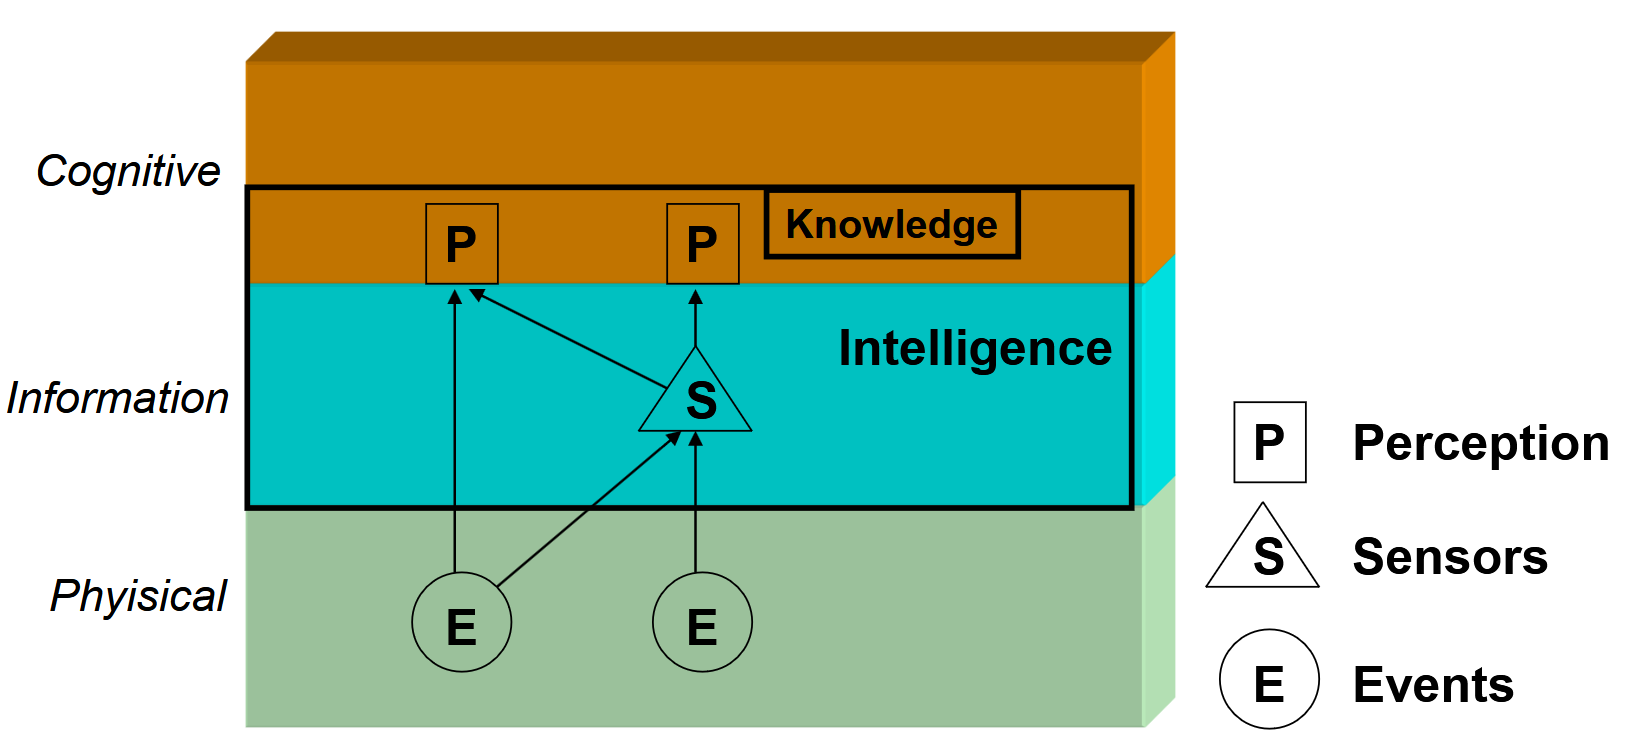
\includegraphics[width=0.45\columnwidth]{images/01/producingCS1.png}
   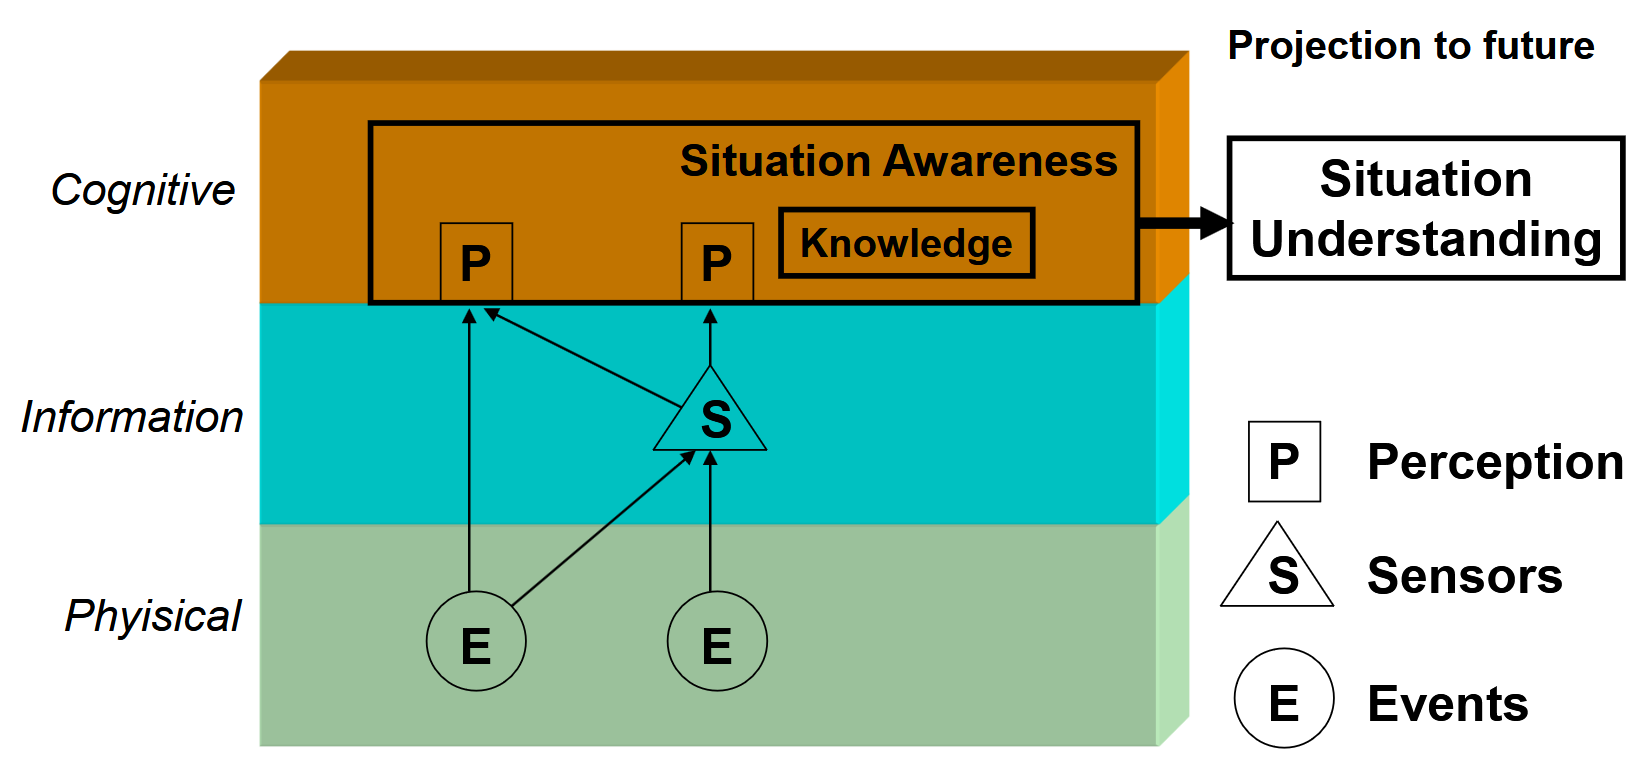
\includegraphics[width=0.45\columnwidth]{images/01/producingCS2.png}
   \caption{Producing Cyber Situational Awareness}
   \label{fig:01/producingCS}
\end{figure}


\subsection{Situational Awareness in Cyberspace}
Cyber situational awareness involves three areas:
\begin{enumerate}
	\item Networks and systems - \textit{Network Awareness}
	\item Threats and incidents (including APT and any other kind of attacks) - \textit{Threat Awareness}
	\item Fullfillment of the mission - \textit{Mission Awareness}
\end{enumerate}

\begin{itemize}
	\item Network awareness:
   \begin{itemize}
	\item Assets and configuration management
	\item Vulnerabilities auditing
	\item Patch management
	\item Sharing of incident awareness
   \end{itemize}
	\item Threat awareness
   \begin{itemize}
	\item Internal incidents and suspicious behavior tracking
	\item Knowledge of external threats, by mean of intelligence activities
	\item HUMINT, OSINT, SIGINT)
	\item Share threat intelligence with goverment organizations (CERTs) or
industry associations
   \end{itemize}
	\item Mission awareness:
   \begin{itemize}
	\item Develop a Common Operational Picture to understand all
dependences and components to operate/develop missions in
cyberspace
	\item Select the best response deccisions during incident management
	\item Risk assesment before any response task execution
	\item Find out mission impact during forensic analysis, after incident
	\item Ellaborate defense plannig for future incidents management
   \end{itemize}
\end{itemize}

Situational awareness can be generated at three traditional military command and control \textbf{levels}:
\begin{enumerate}
	\item \textbf{Tactical}\\
	The main goal at this level is to visualize and take care of events and situations related with assets.\\
   Sometimes this is called also \textit{Technical level}

	\item \textbf{Operational}\\
	Main goal at this level is to summarize tactical level details and putting them in context of impact to organization misión.
	\item \textbf{Strategical}
\end{enumerate}

Es fundamental cabir que la ciberconciencia situational se puede costruir a partir desde cuatro fuentes de información de cyber intelligence techniques:
\begin{figure}[htbp]
   \centering
   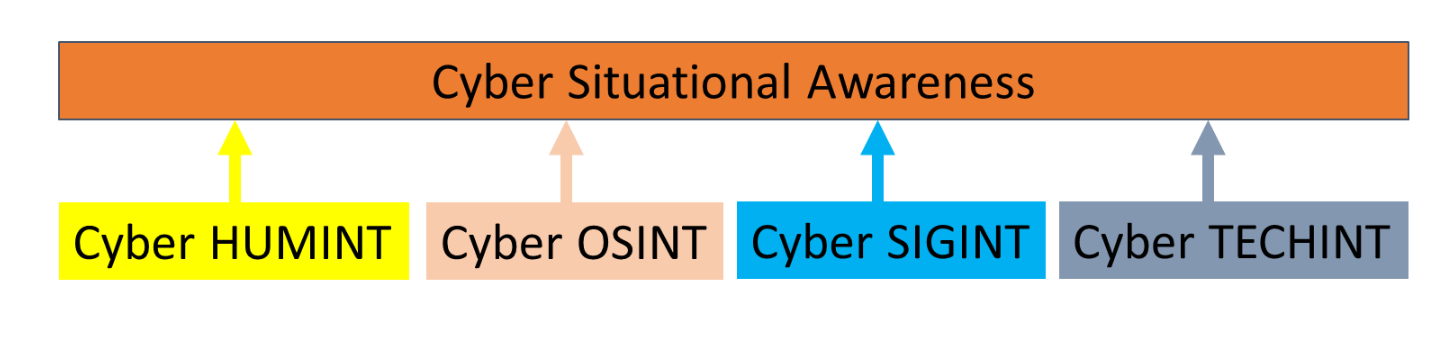
\includegraphics{images/01/CS_CI.png}
   \caption{Cyber intelligence techniques}
   \label{fig:01/CS_CI}
\end{figure}

\begin{itemize}
   \item Cyber \texttt{HUMINT} - Human Intelligence, una fuente de información, por ejemplo, son \textit{usuarios}, que proporcionan información sobre los seres humanos
   \item Cyber \texttt{OSINT} - Open Source Intelligence
   \item Cyber \texttt{SIGINT} - Signal Intelligence
   \item Cyber \texttt{TECHINT} - Technical Intelligence 
\end{itemize}

% VesselFinder es una aplicación que permite visualizar los barcos en tiempo real. Es un ejemplo de visualización de la información.
% Da esta visualización podemos sacar algunas conclusiones, por ejemplo, cuáles son las rutas más transitadas

\section{Ciberconciencia situacional}
Aparte del conocimiento de la situación en general, ahora podemos centrarnos en lo que ocurre en el \textit{ciberespacio}. Esto se llama \textit{Cyber Situational Awareness}.

Associated información with assets:
\begin{itemize}
   \item \textit{Alarms}
   \item \textit{Events}
   \item \textit{Software}
   \item \textit{Services}
   \item \textit{Plugins}
   \item \textit{Properties}
   \item \textit{Netflow} (this is fundamental for the ciberconciencia situacional)
   \item \textit{Groups}
\end{itemize}

\subsection{Vulnerabilidades}
\begin{definition}
   [Vulnerabilities]
   Security gaps that can be used by potencial attackers
\end{definition}

Vulnerabilidades son asociadas con los \textit{assets}, propios o ajenos. Intrínsecamente todos los assets son propensos a haber vulnerabilidades, ahora o en el futuro, cuando algunos condiciones cambian.\\
Vulns son códifigadas y clasficadas en varios modos:
\begin{itemize}
   \item Attack vectors
   \item Assets affected by X
   \item Exploitation easiness of effort tradeoff
   \item Criticallity
   \item Damage assessment if exploited
\end{itemize}

En general, así come si pueden caracterizar las vulnerabilidades:
\begin{itemize}
   \item Vuln ID
   \item Asset
   \item Scan time
   \item Service
   \item Severity
\end{itemize}

\subsection{Amenazas - Threats}
\begin{definition}
   [Threats]
   Elements that can harm our protected system parts or as a whole. Pueden ser internal o external.
\end{definition}

{Tenemos que caracterizar amenazas como:\ns
\begin{itemize}
   \item Kind
   \item Impact
   \item Probability
   \item Origin
\end{itemize}}

MITRE es la más conocida organización que se dedica a la ciberconciencia situacional, y que ha desarrollado un framework para la ciberconciencia situacional.
La MITRE attack matrix es una herramienta que permite visualizar las amenazas y los ataques que se pueden producir en un sistema.

Una amenazas no es sinonimo de \textit{incidente}, que tiene una definición dedicada.
\begin{definition}
   [Incident]
   Un incidente es un evento que supera cierto umbral de peligro
\end{definition}



